
\documentclass{IOS-Book-Article}

\usepackage{mathptmx}
\usepackage{graphicx}
\usepackage{listings}
\usepackage{booktabs}
%\usepackage{times}
%\normalfont
%\usepackage[T1]{fontenc}
%\usepackage[mtplusscr,mtbold]{mathtime}
%
\def\hb{\hbox to 10.7 cm{}}

\begin{document}

\pagestyle{headings}
\def\thepage{}

\begin{frontmatter}              % The preamble begins here.


%\pretitle{Pretitle}
\title{Solving Sparse Linear Systems of Equations using CAF}

%\markboth{}{September 2016\hb}
%\subtitle{Subtitle}

\author[A]{\fnms{Ambra} \snm{Abdullahi Hassan}%
},
\author[A]{\fnms{Valeria} \snm{Cardellini}}
and
\author[B]{\fnms{Salvatore} \snm{Filippone}}

\address[A]{University of Rome Tor Vergata}
\address[B]{Cranfield University}

\begin{abstract}
Fortran Coarrays (CAF) has been part of the Fortran standard since Fortran 2008 and it provides a syntactic extension of Fortran to support parallel programming.
Although MPI is the de facto standard for parallel programs running on distributed memory systems and few scientific softwares are written in CAF, many scientific applications could benefit from the use of CAF. 
We present the migration from MPI to CAF of the libraries PSBLAS  and MLD2P4 for the solution of large systems of equations using iterative methods and preconditioners. 
In this paper we describe the best-usage strategies implemented in PSBLAS and MLD2P4 and we show some performance results obtained on linear systems arising from discretization of 2D and 3D PDEs.  
\end{abstract}

\begin{keyword}
\end{keyword}
\end{frontmatter}

%\markboth{September 2016\hb}{September 2016\hb}
%\thispagestyle{empty}
%\pagestyle{empty}


\section{Introduction}

Fortran has been and still is a dominant language in High Performance Computing. In past decades, Fortran has greatly developed,  and now supports class abstraction, object-oriented programming, pure functions, and coarrays~\cite{Metcalf:2011:MFE}. 
Fortran Coarrays (CAF) has been part of the Fortran standard since Fortran 2008 and it provides a syntactic extension of Fortran to support parallel programming.  
Following Partitioned Global Address Space programming model, with CAF the program is replicated among a certain number of images, executing asynchronously.
Combining, elegancy and simplicity, CAF allows easily for one-sided communications, potentially reducing synchronization and code complexity.
CAF is a language-based approach, which means it is bounds on specific compilers: when a good implementation is available, compiler can concurrently consider serial aspects and communication for optimization. Additionally, if vendors compiler provides support for OpenAcc, the user can easily get a dual benefit form the combined use of CAF and GPUs.  
MPI (Message Passing Interface) defines a suite of functions for communication exchange between processes. Differently from CAF, it is library-based: it means that while independent from a specific compiler, the user is bound to the vendor's fine-tuning of the MPI library~\cite{Garain:2015}.
Although MPI is the de facto standard for parallel programs running on distributed memory systems and few scientific softwares are written in CAF, we think that many scientific applications could benefit from the use of CAF. For this to be possible, studies have to be carried on the impact of CAF on performances and quality of scientific softwares.
In this paper we focus on the solution of large and sparse linear systems of equations and we propose the migration of the PSBLAS~\cite{PSBLAS} and MLD2P4~\cite{mld-toms} libraries. 
The first one implements various iterative solvers while the second exploits most of the communications subroutines in PSBLAS to implement multigrid preconditioners. Using the combinations of the two libraries, we can compare performances of real-world problems in MPI and in CAF.
Few attempts to implement multigrid solvers in CAF have been made, for example in~\cite{Numrich:1998} (in which early versions of CAF and MPI have been used).  In~\cite{Garain:2015} a comparison between MPI3 and CAF is presented for spectral techniques, multigrid techniques and for applications drawn from computational fluid dynamics. It shows that Cray implementations of MPI3 and CAF performances in message passing are comparable (with CAF slightly outperforms MPI3 in some cases), and it points out the advantages of CAF when it comes to ease of implementation.
In this paper we compare performances of CAF and MPI on problems arising from discretization of 2D and 3D PDEs, using preconditioned iterative methods (also with multigrid preconditioners). We used the GNU compiler and the OpenCoarray library~\cite{PGAS14}, both opensource and easily accessible.
\section{Fortran Coarray}
Coarray Fortran extends Fortran language with minimal syntactic constructs, allowing for Single Program Multi Data (SPMD) parallel programming. 
It follows the Partitioned Global Address Space (PGAS) parallel programming model, which it is an effective alternative combining the advantages of the SPMD programming style for distributed memory systems with the data referencing semantics of shared memory systems. 
In PGAS model threads share the global address space, each having a portion of space which is local to it. 
Besides CAF, Unified Parallel C (UPC)~\cite{UPCSpec}, Chapel~\cite{chapel}, X10~\cite{Charles:2005} and SHMEM are all based on the PGAS model.
With CAF, Fortran users do not need to invoke subroutines from an  external API (as in MPI), nor preprocessing directives (as in OpenMP) to create parallel programs. 
Since most of the parallel bookkeeping is handle behind the scene by the compiler, CAF achieves a good trade-off between readability and performance and compared to MPI the parallelization is easier to follow, the code is shorter and less complex. We can think, for example, of the burden of passing a non-contiguous array using MPI   or to the fact that with CAF there is no need to write separate code for sending and receiving a message.
Coarrays are fully supported by Cray and Intel compilers. Although GNU compilers provide only partial coarray support  (only single image),  the open source openCoarrays project provides two coarray transport layers based on MPI and on GASNet~\cite{PGAS14}. 

In CAF the program is replicated a fixed number of times and each replication (called images) executes asynchronously having its own set of data objects. 
Some variables can be declared as coarrays through the use of coindices (indicated by square brackets) with a syntax very similar to normal Fortran array syntax. 
\begin{lstlisting}
integer ::co_a[*],co_b(n,m)[*]
\end{lstlisting}

Coarrays can be accessed by the other images, thus enabling data exchange. 

\begin{lstlisting}
co_a[1]=co_a
\end{lstlisting}

Each image is assigned a unique index, through which the programmer can control the flow of the execution. Image indices start from 1 (not from 0 as MPI process ranks) and can be retrieved using the intrinsic function $this\_image()$. The number of total images can be retrieved using the function $num\_images()$. The total number of images can be different from the total number od processors and it can be decided at compile, link or runtime depending on the implementation. 

CAF communications are synchronous and non-blocking. 
To avoid deadlock and race conditions, the programmer has to ensure consistency through the use of synchronization statements.
The sync all statement corresponds to a global barrier (all images waiting for each tohers) while $sync images$ allows for explicit synchronization of single images. Moreover, with CAF events, an image can use an event post statement to notify another images or it can wait for an event posted by another image before continuing execution. This allows for more sophisticated synchronization strategies.  

Other than explicit synchronization, in a CAF program there can be implicit synchronization points. The programmer must be aware of this, because they can lead to a drastic change in performance.
An example of an implicit synchronization point is allocation or deallocation of an allocatable coarray:

\begin{lstlisting}
integer, allocatable :: co_a(:,:)[:]
allocate(co_a(i,10)[*])
\end{lstlisting}

Of course, for code between synchronizations, the compiler can use the usual optimization techniques as if only one image is present~\cite{CAF}.

\section{PSBLAS and MLD2P4}

Most of scientific and engineering applications require solving a large sparse linear system of equations efficiently on parallel machines.  
In these cases direct solvers such as Gaussian elimination are usually ineffective and iterative solvers are preferred.
These techniques produce a sequence of approximate solutions, ideally converging to the real one. Rate of convergence of iterative methods depends upon the condition number of the matrix, hence iterative methods usually involve a transforation of the original matrix into a more well-conditioned one. This transformation is called a preconditioner ~\cite{barrett1994templates}. Among iterative methods, Krylov methods are based on minimizing the residual over a Krylov subspace and are considered among the most important \cite{ipsen1998idea}. The Conjugate Gradient (CG) \cite{shewchuk1994introduction}, the Generalized Minimal Residual (GMRES) \cite{saad1986gmres} and the Biconjugate Gradient (BiCG) \cite{van1992bi} are all Krylov methods. 
Multigrid methods have also shown promising results in solving linear systems arising from partial differential equations and they have the nice property that they can achieve convergence rates which are, in theory, independent of the mesh size ~\cite{saad2003iterative}.
Multigrid can be used as stand-alone solvers ~\cite{brandt1977multi} or as preconditioner for a Kylov subspace method ~\cite{bramble1990parallel}.
PSBLAS is a library of Basic Linear Algebra Subroutineas for parallel sparse applications is designed to handle parallel implementation of iterative solvers for sparse linear systems. It is implemented if object-oriented Fortran 2003. The serial computations are based on the serial sparse BLAS ~\cite{duff2002overview}, while the inter-process massage exchanges are encapsulated in an application layer inspired by the Basic Linear Algebra Communication Subroutines (BLACS) library ~\cite{whaley1997user}. PSBLAS library contains, among the others, subroutines for sparse-matrix-by-dense-matrix multiplication, sparse triangular system solution, dot product, sparse matrix and data distribution preprocessing.
While addressing a distributed memory execution model the current PSBLAS design does not preclude different implementation pradigms.
MLD2P4 (Multi-level Domain Decomposition Parallel Preconditioners Package based on PSBLAS) is a package for parallel algebraic multilevel preconditioners. A purely algebraic approach is used and no information about the underlying physical grid is needed to build the preconditioner. MLD2P4 preconditioner are intended to be used in conjuction with the iterative solvers available in the context of PSBLAS. 
Since in MLD2P4 inter-process data communiations is managed through PSBLAS, writing a CAF version give us dual benefit:

\begin{enumerate}
\item First, we can compare MPI and CAF on Krylov subspace methods and simple preconditioners, usign PSBLAS
\item Secondly, we can compare MPI and CAF on multilevel preconditioners, since MLD2P4 data communication is actually managed on PSBLAS.
\end{enumerate}  

Additionally, since both PSBLAS and MLD2P4 are open source, once the CAF version is released CAF programmers will be able to use them inside their scientific application.

 
\section{Implementation}
We converted the PSBLAS code gradually from MPI to CAF, thus having the two communication strategies coexisting in the same code. 
We detected three communication patterns to modify:

\begin{enumerate}
\item The halo exchange
\item Collective subroutines
\item Point-to-point communication in data distribution
\end{enumerate}

In the following, we address the three of them separately.

\subsection{Halo Exchange}

In PSBLAS~\cite{PSBLAS}, data distribution is performed keeping in mind the underlying physical problem, such as the discretization mesh of the PDE. 
Each point in the discretization mesh corresponds to a variable and, consequently, to an index in the coefficient matrix. We say that index $i$ depends upon index $j$ if $a_{ij}\neq0$. 
In the process of distributing data among processes, the original domain is divided into subdomains. 
In each subdomain a boundary point is a point depending on points from different domains. An halo point is the one for which there is at least one boundary point in another domain depending upon it. 
This means that when performing matrix and vector operations (such as a matrix-vector production), halo points will be requested by other processes and the amount of exchanged data is given by the cardinality of the boundary points. 
Every time this happens we perform a so-called halo exchange operation. We can think of halo exchange as a sparse all-to-all communication (or as an MPI\_ALLTOALLV operation, in MPI jargon).
\begin{figure}
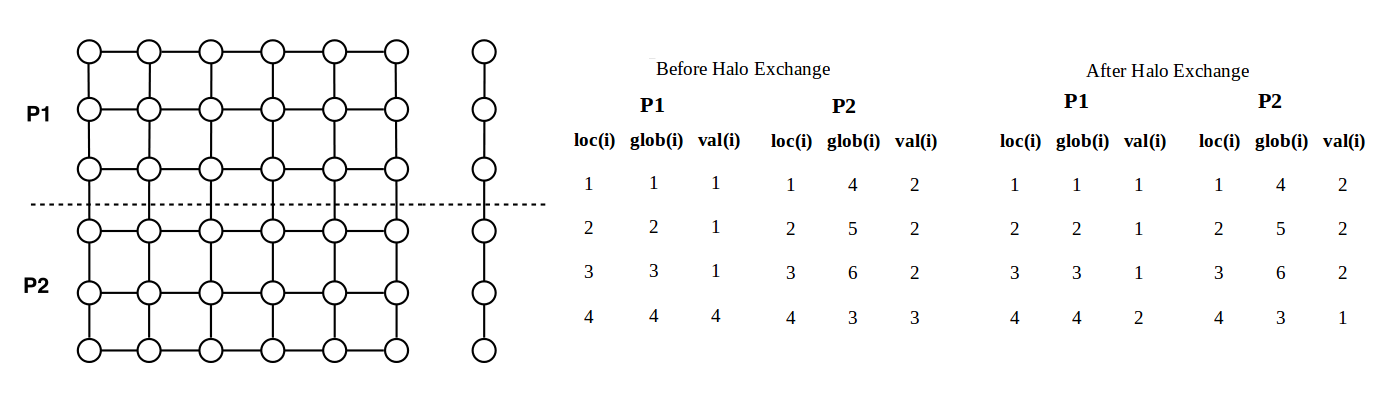
\includegraphics[height=1.5in, width=4.65in]{halo2.png}
\caption{Example of halo exchange on 2 images. }
%\label{classes}
\end{figure}
In order to obtain better performances in PSBLAS halo exchange is actually reimplemented in terms of point-to-point operations. 
The subroutine performing the exchange takes a list of dependencies as input. The list consists of variable size blocks, one for each of the communication to perform. The list terminates with $-1$ and each block consist of several elements:
\begin{enumerate}
\item The first entry identifies the process to which exchange data.
\item The number of elements to receive
\item The local indices of the elements to receive
\item The number of elements to send
\item The local elements to send
\end{enumerate}
The order of the blocks, determining the order in which communications take place, is defined through an internal algorithm.
For the MPI version we can choose between different strategies by setting a suitable flag as an input variable. The halo\_exchange can thus happen through a call to MPI\_ALLTOALLV, by using send and receives communications in synchronized pairs, by performing only a send or a receive (in this case, the code needs to complete the communication by calling the same subroutine with the complementary communication in a later stage) or by using mpi\_irecv and mpi\_send. 
The latter choice is the standard one, since it leads to the best results in terms of performance. In this case data exchange actually takes place through the use of two buffers (snd\_buf and rcv\_buf) according to the following flow:
\begin{enumerate}
\item pack data into the snd\_buffer
\item call the non-blocking mpi\_irecv using rcv\_buffer as output
\item complete the exchange calling blocking mpi\_snd using snd\_buffer as input
\item upack data from the rcv\_buffer
\end{enumerate} 

When rewriting the halo exchange subroutine in CAF, we need to choose if we want to perform the exchange operation using GET or PUT operations. 
Let's assume that we need to pass a scalar value, stored on the variable $a$ from image $1$ to image $2$. Since communications in CAF are one-sided, this can be done in two ways:

\lstset{language=Fortran} 

\begin{lstlisting}
if (this_image()==1) a[2] = a
\end{lstlisting}
or
\begin{lstlisting}
if (this_image()==2) a = a[1]
\end{lstlisting}

In the first case image $1$ performs a PUT operation; in the second case, image $2$ performs a GET operation. We implemented both cases in PSBLAS, but preliminary tests  show that PUT leads to a slightly smaller execution time.
Both versions require a coarray buffer. In the GET version it is possible to incorporate the data exchange in the operation of packing the sending data: in this case no other buffer is needed. For the PUT version instead, the rcv\_buf is still present.
A key factor is the management of  allocation of coarrays in the code. Since in CAF allocate and deallocate statements are implicit synchronization barriers, for the sake of performance they should be avoided unless strictly necessary.
For this reason in PSBLAS code we declared the coarray buffer with the save attribute and we reallocate it only when the actual amount of data to exchange does not fit the current size:

\lstset{language=Fortran} 
\begin{lstlisting}
  if (psb_size(buffer) < xchg%max_buffer_size) then
    if (allocated(buffer)) deallocate(buffer)
    allocate(buffer(xchg%max_buffer_size)[*],stat=info)
    if (allocated(sndbuf)) deallocate(sndbuf)
    if (info == 0) allocate(sndbuf(xchg%max_buffer_size),stat=info)
    if (info /= 0) then
      info = psb_err_internal_error_
      call psb_errpush(info,name,a_err='Coarray buffer allocation')
      goto 9999
    end if
  end if
\end{lstlisting}

Note that with MPI, the opposite is true: we deallocate the buffers as soon as we can, in order to save run-time memory.
Before performance results are shown for the halo exchange, we can make a comparison between MPI and CAF for the halo exchange in terms of impact on software quality.
The interface for the halo exchange in psblas is psi\_swapdata. This interface requires 5 implementations for each of the available datatypes in PSBLAS (integer, real, double precision, complex and double precision complex). Each of them needs to be implemented for the the real vector, the real matrix and the two derived types defined in PSBLAS psb\_X\_vect and psb\_X\_multivect. A second interface, psi\_swaptran performs a transpose halo exchange. As a consequence, we need 40 implementations of the halo exchange: these are all very similar with some minor modifications. It is clear that any impact on the code, although relatively small on the single implementation, has to be multiply by 40. 
Keeping this in mind, we detected two differences between the MPI and the CAF version:

\begin{enumerate}
\item number of input variables: the MPI version requires 12 input variables, while the CAF version requires 8 input variables
\item the number of lines of code for the single implementation is 185 for MPI and 116 for CAF 
\end{enumerate}

Less input parameters results in a more clear interface, and we get a significant reduction in the number of lines of the code (regarding only the halo exchange).
  
\subsection{Collective Subroutines and Point-to-point in Data Distribution}

Here we take into account all the subroutines performing collective communications, in which all images take part in the communication. While rewriting the halo exchange using CAF leads to a reduction in the number of lines in the code, in this case we can expect an increasing in the length of the code. This is because MPI provides an interface for most of the collectives we may need in solving a sparse linear system in parallel. For CAF collective subroutines are reduced in number; they are:

\begin{enumerate}
\item co\_broadcast
\item co\_max
\item co\_min
\item co\_sum
\item co\_reduce
\end{enumerate}

They involve synchronization within them, but not at the start or at the end.  
With CAF, we need to write from scratch some of the collective subroutines we need.
We do this in the psb\_caf\_mod. In this module, we have the implementations for the interfaces caf\_scatterv, caf\_gatherv, caf\_allgatherv, caf\_allgatherv caf\_gather, caf\_alltoallv and caf\_alltoall. 
As an example, the code for the caf\_alltoall has been provided. 
\lstset{language=Fortran} 
{\small
\begin{lstlisting}
  subroutine caf_alltoall(snd,rcv, m, info)
    implicit none
    integer(psb_ipk_), intent(in) :: m
    integer(psb_ipk_), intent(in) :: snd(:)
    integer(psb_ipk_), intent(out):: rcv(:), info
    !Local
    integer(psb_ipk_) :: me, np,i, snd_start, snd_finish, snd_tot
    integer(psb_ipk_), allocatable :: buffer(:)[:], rcv_start, rcv_finish
    if ( m < 0) then
      print*,'Error, m must be greater or equal to zero'
      info = -1
    endif
    me = this_image()
    np = num_images()
    snd_tot=m*np
    if (allocated(buffer)) deallocate(buffer)
    allocate(buffer(snd_tot)[*], STAT = info)
    if (info /= 0) then
       print*,'allocation error', info
       return
    endif
    rcv_start = (me-1)*m +1
    rcv_finish = rcv_start + m - 1
    do i=1,np
      snd_start = (i-1)*m +1 
      snd_finish = snd_start + m - 1
      if (rcv_finish > snd_tot) then
        print*,'Error, rcv_finish > snd_tot'
        info = -2 
	return
      endif
      if (snd_finish > size(snd,1)) then
        print*,'Error, snd_finish > size(snd,1)'
        info = -3 
      endif
      buffer(rcv_start:rcv_finish)[i]=snd(snd_start:snd_finish)
    enddo
    !sync to ensure all image has finishe the PUTs 
    sync all
    rcv(1:snd_tot)=buffer(1:snd_tot)
    if (allocated(buffer)) deallocate(buffer)
  end subroutine caf_alltoall
\end{lstlisting}}
For what it concerns the reduce operations, we show a comparison between CAF and MPI based on the code for the reduce operation based on the norm2. 
First, the code for the MPI version:
\begin{center}
{\small
\begin{lstlisting}


call psb_realloc(size(dat),dat_,iinfo)
dat_ = dat
if (iinfo == psb_success_) &
    & call mpi_allreduce(dat_,dat,size(dat),psb_mpi_r_dpk_,&
    & mpi_dnrm2_op,ictxt,info)

\end{lstlisting}}
\end{center}

And the code the CAF version: 

\begin{center}
{\small
\begin{lstlisting}

call co_reduce(co_dat_,caf_dnrm2)

\end{lstlisting}}
\end{center}
In this case the CAF syntax is more compact and there is no need to use the extra euxiliary variable dat\_.
Finally, we modified the psb\_matdist subroutines, an utility subroutine that uses point-to-point communications to distribute a matrix among processors according user defined data distribution. In this case, for both MPI and CAF we are using one-sided communications. In the case of CAF, to ensure performance optimizations, we used events to ensure synchronization among images. 
\section{Results}
CAF and MPI versions of PSBLAS and MLD2P4 have been tested on matrices generated by 2D and 3D PDEs.
The experiments were carried out on the Yoda linux cluster, operated by the Naples Branch of the CNR Institute for High-Performace Computing and Networking. Its compute nodes consist of 2 Intel Sandy Bridge E5-2670 8-core processors and 192 GB of RAM, connected via Infiniband.
Both PSBLAS, MLD2P4 and OpenCoarrays-1.9 have been compiled on the top of MPICH-3.2 and GNU 7.1.

In PSBLAS and MLD2P4 it is possible to create the matrix corresponding to the PDE $
-a_1\frac{\mathrm d}{\mathrm d x \mathrm d x} \left(u \right) -a_2\frac{\mathrm d}{\mathrm d y \mathrm d y} \left(u \right) +b_1\frac{\mathrm d}{\mathrm d x} \left(u \right) +b_2\frac{\mathrm d}{\mathrm d y} \left(u \right) +cu = f
$ for the 2D problem and $
-a_1\frac{\mathrm d}{\mathrm d x \mathrm d x} \left(u \right) -a_2\frac{\mathrm d}{\mathrm d y \mathrm d y} \left(u \right) -a_3\frac{\mathrm d}{\mathrm d z \mathrm d z} \left(u \right) +b_1\frac{\mathrm d}{\mathrm d x} \left(u \right) +b_2\frac{\mathrm d}{\mathrm d y} \left(u \right) b_3\frac{\mathrm d}{\mathrm d z} \left(u \right)
 + cu = f$ for the 3D problem. The user can set the parameter $idim$. The dimension of the grid is then $idim^2$ for the 2D case and $idim^3$ for the 3D case.
 The resulting linear system is solved using a Biconjugated Conjugate Gradient Stabilized (BiCGSTAB) with a Block Jacobi preconditioner. The iterations are stopped when the 2-norm of the residuals vector achieved a reduction by a factor of $10^{-9}$
 
First we tested weak scalability for a 2D problem by keeping (roughly) constant the number of lines per process (Table \ref{weak}). 


\begin{table}[]
\centering
\caption{Weak scalability test for a 2D problem ($a_1=a_2=\frac{1}{80}$, $b_1=b_2= \frac{1}{\sqrt{2}}$,  $c=0$ dim = $idim^2$)}
\label{weak}
\begin{tabular}{@{}rrrrr@{}}
\toprule
\multicolumn{1}{c}{np} & \multicolumn{1}{c}{idim} & \multicolumn{1}{c}{MPI} & \multicolumn{1}{c}{\begin{tabular}[c]{@{}c@{}}CAF \\ ($sync images$)\end{tabular}} & \multicolumn{1}{c}{\begin{tabular}[c]{@{}c@{}}CAF\\ (events)\end{tabular}} \\ \midrule
1                      & 250                      & 0.64                 & 0.90                                                                          & 0.89                                                                    \\
2                      & 350                      & 0.99                 & 1.03                                                                           & 1.0                                                                      \\
4                      & 500                      & 1.37                  & 1.58                                                                           & 1.33                                                                     \\
8                      & 700                      & 2.00                  & 2.20                                                                           & 3.88                                                                     \\
16                     & 1000                     & 3.03                  & 3.82                                                                           & 4.41                                                                     \\
32                     & 1400                     & 5.07                  & 5.36                                                                           & 6.10                                                                     \\
64              

      & 2000                     & 6.52                  & 6.81                                                                           & 7.79                                                                     \\ \bottomrule
\end{tabular}
\end{table}

For CAF, two versions of the halo exchange have been tested: one performing synchronization through the use of events, the other through the use of the $sync images$ statement. While we expected synchronization through events to perform better, we actually observed that the version with $sync images$ is faster especially on many processes. In this case, MPI and CAF versions have total execution times that are very similar. 
Secondly, strong scalability tests have been performed for both 2D and 3D problems. Again, halo exchange with sync images performs better: for this reason in the following we show only results for this case. Table \ref{strong} shows results for the 3D problem.
 
\begin{table}[]
\centering
\caption{Strong scaling for a 3D problem: BiCGSTAB with BJAC preconditioner ($a_1=a_2=a_3=\frac{1}{80}$, $b_1=b_2=b_3=\frac{1}{\sqrt{3}}$, $c=0$,$idim=200$}
\label{strong}
\begin{tabular}{@{}rrr@{}}
\toprule
\multicolumn{1}{c}{np} & \multicolumn{1}{c}{MPI} & \multicolumn{1}{c}{CAF} \\ \midrule
1                      & 88.7                  & 106                  \\
2                      & 46.3                  & 46.5                  \\
4                      & 34.9                  & 23.3                  \\
8                      & 1.72                  & 1.45                  \\
16                     & 7.31                  & 9.94                  \\
32                     & 5.71                  & 5.12                  \\
64                     & 4.04                  & 3.61                  \\ \bottomrule
\end{tabular}
\end{table} 

Finally, we show results for the 3D problem, using the multilevel preconditioner implemented in MLD2P4. BiCGSTAB is used, with a multiplicative multilevel preconditioner, smoothed decoupled aggregation algorithm. The iterations are stopped when the 2-norm of the residuals vector achieved a reduction by a factor of $10^{-6}$ and a Jacobi smoother is used. The coarsest level matrix is distributed among processes and an incomplete LU factorization is used to solve the coarsest level matrix. Results are shown in Table \ref{Strong2}. Again performances of MPI and CAF are comparable in term of execution time. In the table, both the preconditioner building time (tprec) and the solution time are shown (tsolve). 

\begin{table}[]
\centering
\caption{Strong scaling for a 3D problem: BiCGSTAB with with a 2 level preconditioner ($a_1=a_2=a_3=1$, $b_1=b_2=b_3=0$, $c=0$,$idim=200$}
\label{Strong2}
\begin{tabular}{@{}rrrll@{}}
\multicolumn{1}{l}{}   & \multicolumn{2}{c}{MPI}                                & \multicolumn{2}{c}{CAF} \\ \midrule
\multicolumn{1}{c}{np} & \multicolumn{1}{c}{tprec} & \multicolumn{1}{c}{tsolve} & tprec      & tsolve     \\ \midrule
1                      & 37.5                      & 35.8                       & 37.4       & 35.6       \\
2                      & 19.9                      & 27.1                       & 19.8       & 26.9       \\
4                      & 10.3                      & 15.5                       & 10.5       & 15.3       \\
8                      & 5.56                      & 8.46                       & 5.37       & 9.87       \\
16                     & 3.71                      & 5.64                       & 2.35       & 5.87       \\
32                     & 2.19                      & 3.68                       & 2.44       & 3.72       \\
64                     & 1.45                      & 4.0                        & 2.12       & 3.72       \\ \bottomrule
\end{tabular}
\end{table} 
  
\section{Conclusions}

We successfully migrated PSBLAS library from MPI to CAF. Since MLD2P4 communication is based on the PSBLAS framework, most of MLD2P4 preconditioners can exploit underlying CAF communication with little effort. We point out that in the migration from MPI to CAF we retained as much as the original code and structure that we could. While this can lead to CAF code which is not as clear and readable as it would be if the original software was thought and written in CAF from the beginning, we think that the previous examples show the capability of CAF to express parallelism in a simpler way than MPI. In all cases, CAF code is shorter, clearer and easier to read. However, the CAF programmer need to provide an interface for most of MPI collective subroutines, which can increase the lenght of the code. 

Performance is a key factor, so we tested both the MPI and CAF versions on problems arising from discretization of 2D and 3D PDEs. Neither CAF nor MPI version has shown a clear superiority in terms of performance, with execution time almost identical in the two cases. So, the migration from MPI to CAF did not lead to a loss of performance.
Additionally, we provided few examples of how CAF programmer choices can affect performance (for example: "get" versus "put" for one-sided communication, events versus $sync images$ for synchronization, clever coarrays allocation).
  
 
 
\bibliographystyle{unsrt}
\bibliography{psblas-caf}

\end{document}
 
\begin{thebibliography}{99}
\bibitem{r6}
Numrich, Robert W., and John Reid. "Co-Array Fortran for parallel programming." ACM Sigplan Fortran Forum. Vol. 17. No. 2. ACM, 1998.
\bibitem{r7}
Metcalf, Michael, John Reid, and Malcolm Cohen. Modern Fortran Explained. Oxford University Press, 2011.
\bibitem{r8}
UPC Consortium. UPC Language Specifications, v1.2.
Tech Report LBNL-59208, Lawrence Berkeley
National Lab, 2005.
\bibitem{r10}
V. Saraswat, B. Bloom, I. Peshansky, O. Tardieu, and
D. Grove. The X10 language specification, v2.2.3,
2012.
\end{thebibliography}

